\documentclass[10pt,a4paper]{article}
\usepackage[T1]{fontenc}
\usepackage{lmodern}
\usepackage[utf8]{inputenc}
\IfFileExists{french.ldf}{\usepackage[french]{babel}}{\usepackage[french,provide=*]{babel}}
\ifdefined\frenchsetup\frenchsetup{AutoSpacePunctuation=false}\fi
\usepackage[margin=2cm]{geometry}
\usepackage{amsmath,amssymb,booktabs,tabularx,longtable,array}
\usepackage[expansion=false]{microtype}
\usepackage{xcolor}
\usepackage{graphicx}
\usepackage{tikz}
\usetikzlibrary{arrows.meta}
\usepackage{listings}
\usepackage[hidelinks]{hyperref}
\hypersetup{pdftitle={UrbanFlow : plateforme d'analyse des trajets de taxis},pdfauthor={Ion Cazacu, Théo Delias},pdfsubject={Rapport de projet, M2 SLCD}}
\usepackage{fancyhdr}
\usepackage{enumitem}
\setlist{nosep,leftmargin=*}
\setlength{\parindent}{0pt}
\setlength{\parskip}{4pt}
\setlength{\emergencystretch}{2em}
\pagestyle{fancy}\fancyhf{}\fancyhead[L]{UrbanFlow --- Rapport de projet}\fancyfoot[C]{\thepage}
\setlength{\headheight}{13pt}
\lstset{basicstyle=\ttfamily\scriptsize,breaklines=true,columns=fullflexible,keepspaces=true,frame=single,showstringspaces=false}
\newcommand{\code}[1]{\texttt{\detokenize{#1}}}
\newcommand{\chemin}[1]{\texttt{\path{#1}}}
\title{\vspace{-1.2cm}UrbanFlow\\\large Analyser la mobilité urbaine à partir des trajets de taxis jaunes de New York}
\author{Ion Cazacu et Théo Delias --- Master 2 SLCD, Big Data et NoSQL}
\date{8 novembre 2026}
\begin{document}
\maketitle\vspace{-1.0cm}
UrbanFlow répond à six services (F1 à F6) par une API REST au-dessus de MongoDB.
Nous avons comparé trois déploiements sur les mêmes 20\,332\,093 lignes TLC de janvier
à juin 2024 : un serveur local, deux shards par zone de départ et deux shards par
période. Les 13 requêtes de la comparaison automatique donnent des réponses identiques
partout. Le placement par zone raccourcit tous les mélanges de E3 de 17 à 33\,\% par
rapport au local, et coûte 42\,\% de stockage en plus et, sur la charge large, 25\,\%
de CPU en plus. Le placement par période termine la charge large 7\,\% plus vite, mais
il est le plus lent sur les zones chargées et sur F5 à l'échelle de la ville (59 s contre
22 s). La perte d'un shard rend indisponibles les requêtes qui en ont besoin : l'API
renvoie alors une erreur 503 et ne présente jamais de résultat partiel.

\section{Périmètre et organisation du travail}
UrbanFlow analyse les enregistrements de trajets des taxis jaunes de New York.
Le jeu initial couvre janvier, février et mars 2024, dont le changement d'heure
du 10 mars. Avril est réservé à la mise à jour F6 ; mai et juin complètent les
six mois prévus pour les expériences. Brooklyn sert de point d'appui aux exemples,
mais les données de toute la ville sont conservées. Les trajets enregistrés ne
permettent pas de mesurer une demande non satisfaite ni l'ensemble des déplacements
new-yorkais : les résultats portent sur cette archive de taxis \cite{sujet}.

Nous nous sommes réparti le travail : Théo s'est occupé de la récupération des données, de leur qualité, du modèle, de l'API locale et des services F1 à F5, et Ion de F6, des déploiements répartis, des expériences E1-E3 et de leur analyse. Pour la partie données et F1-F5, 
Codex a été utilisé pour développer et expliquer du code, préparer des vérifications et
rédiger. 



\section{Données et règles de qualité}\label{sec:donnees}
Les sources sont les Parquet mensuels \emph{Yellow Taxi Trip Records} et le
référentiel officiel des zones TLC. Le manifeste donne pour chaque fichier son
URL, sa date de récupération, sa taille et son SHA-256. Nous avons récupéré les fichiers de janvier à avril le 2 novembre 2026 et ceux de mai et juin le 3 novembre ;
les empreintes complètes sont dans \chemin{data/manifest.json} \cite{tlc,preuves}.

\begin{center}\small
\begin{tabular}{lrrrr}
\toprule
Fichier 2024 & Lignes sources & Profil activity & Profil flows & Profil journey\\
\midrule
Janvier & 2\,964\,624 & 2\,929\,120 & 2\,898\,055 & 2\,841\,251\\
Février & 3\,007\,526 & 2\,971\,445 & 2\,942\,952 & 2\,878\,111\\
Mars & 3\,582\,628 & 3\,538\,317 & 3\,503\,542 & 3\,420\,628\\
Avril & 3\,514\,289 & 3\,470\,540 & 3\,435\,410 & 3\,394\,040\\
Mai & 3\,723\,833 & 3\,674\,841 & 3\,636\,771 & 3\,591\,918\\
Juin & 3\,539\,193 & 3\,490\,398 & 3\,452\,592 & 3\,404\,607\\
\midrule
Total & 20\,332\,093 & 20\,074\,661 & 19\,869\,322 & 19\,530\,555\\
\bottomrule
\end{tabular}
\end{center}
Ces effectifs sont ceux des bilans par fichier : 9\,554\,778 lignes sources pour les
trois mois initiaux, 20\,332\,093 pour les six mois, pas un nombre garanti de
déplacements physiques distincts. À l'import, aucune ligne d'un fichier n'a été
retrouvée dans un autre : la base contient autant de documents que de lignes
sources. Le référentiel contient 265 zones. Dans le fichier de janvier,
25\,258 lignes ont une zone de départ rattachée à Brooklyn ; Manhattan en compte
2\,646\,948 \cite{preuves}.

Une ligne appartient à une période selon sa date réelle de départ, et non selon
le mois du fichier. F1 et F3 en mode arrivées utilisent toutefois la zone \emph{et}
la date d'arrivée. Les intervalles sont semi-ouverts $[d_0,d_1[$ en heure locale
\code{America/New_York}. Cette convention évite de compter deux fois une borne.

Les anomalies de qualité ne provoquent pas de suppression à l'import : elles sont conservées dans
\code{quality_flags}, puis chaque analyse applique son profil.
\code{activity} exclut les montants totaux négatifs et les doublons exacts ;
\code{flows} ajoute les zones 264/265, sans localisation précise ;
\code{journey} ajoute les durées nulles ou négatives, celles au-delà de six heures,
les distances nulles ou supérieures à 100 miles, les vitesses supérieures à
80 miles/h et les heures DST non résolues. Le profil activity sert à F1 et F3, flows à F2 et F5, journey à F4. Ces seuils larges écartent des anomalies
manifestes, sans définir un trajet « normal ». En janvier, le profil journey
écarte 123\,373 lignes, soit 4,16\,\%, contre 1,20\,\% pour activity.
Les motifs peuvent se cumuler ; leur somme n'est pas le total des exclusions.

Un doublon exact est une copie de toutes les colonnes dans un même fichier ;
les deux lignes restent stockées et seule la première entre dans les analyses. Une annulation est repérée par
le fournisseur, les deux horodatages, les zones et un montant opposé ; l'original
positif est conservé. La détection est faite sur le fichier entier avant l'écriture
par lots de 5\,000, ce qui évite de dépendre des frontières de lots, mais impose
un coût mémoire que nous n'avons pas mesuré. Les anomalies ne sont pas toutes
couvertes : le contrôle des zones vise notamment 264/265 et la détection des
annulations reste interne à chaque fichier. L'annexe \ref{ann:qualite} documente
huit anomalies ou particularités effectivement présentes avec leurs lignes sources.

\section{Modèle local et accès à MongoDB}\label{sec:modele}
MongoDB fonctionne comme un serveur séparé dans Docker Compose ; l'application
y accède par une URI réseau. Le déploiement local utilise MongoDB 8.0.16 sur
\code{127.0.0.1:27018}, avec un volume persistant. L'ingestion et les contrôles
Parquet sont en Python. L'API est en Spring Boot 3.5.7, Java 21, avec Spring Data
MongoDB et \code{MongoTemplate}. JPA n'est pas utilisé : les requêtes sont des
filtres et pipelines BSON explicites. Les contrôleurs valident les entrées, les
services appliquent les règles et les repositories interrogent la base. Postman
sert d'interface de démonstration \cite{sujet,code}. Les accès attendus sont des filtres par zone et par
intervalle de dates suivis de regroupements : les index de la section~\ref{sec:mesures}
servent ces filtres. MongoDB offre aussi le partitionnement natif, qui laisse à l'API
une seule URI en déploiement réparti (section~\ref{sec:reparti}).

La collection \code{trips} conserve les colonnes TLC dans \code{data}, la provenance
\code{source.file_id}/\code{source.row_number}, la durée \code{duration_s} et les
flags. \code{zones} associe un identifiant entier aux noms et boroughs : les noms
ne sont pas des clés uniques. \code{imports} conserve le SHA-256 du fichier,
ses métadonnées et son état \code{loading}, \code{failed} ou \code{complete}.
Les services ne sélectionnent que les imports complets. Aucun agrégat matérialisé
n'est nécessaire aux services décrits ici.

\paragraph{Identité et reprise.}
L'identité d'un trajet combine l'heure de départ, une empreinte de toutes les
colonnes canonisées et le rang parmi les lignes identiques du fichier. Le code
utilise une empreinte Pandas de 64 bits, \emph{distincte} du SHA-256 de provenance.
Deux copies dans un fichier ont des rangs différents ; une ligne déjà importée
retrouve son identité et l'index unique \code{_id} empêche sa réinsertion.
L'import utilise des insertions par lots et traite les collisions de clé
comme des lignes déjà présentes.
Cette règle ne résout pas toute ambiguïté : deux enregistrements identiques issus
de fichiers indépendants peuvent être confondus, une correction de contenu
produit une nouvelle identité, et une collision d'empreinte reste possible.
En cas de recouvrement, le document garde la provenance de la première insertion,
pas toutes ses rééditions. La section~\ref{sec:f6} teste cette règle sur de vraies lignes.

\paragraph{Dates et durées.}
Les heures locales TLC sont stockées en chaînes ISO sans fuseau. Les conversions
UTC ne sont que temporaires pour calculer la durée : attribuer New York aux
deux heures, convertir en UTC, puis soustraire. Une arrivée inexistante ou ambiguë
produit \code{null}, pas une durée locale de secours. La ligne 942\,762 de mars
part le 9 mars à 23:38:43 et arrive le 10 à 03:40:14 : la durée réelle est
10\,891 s, contre 14\,491 s par soustraction locale. Elle porte
\code{DST_SPANNING}. La ligne 841\,170 arrive à 02:09:54 le 10 mars, heure qui
n'existe pas : elle porte \code{DST_UNRESOLVED} et est exclue de journey.

\paragraph{Calculs côté serveur et traçabilité.}
\code{$match} filtre les documents ; \code{$project} prépare les champs utiles
sans modifier la base ; \code{$group} regroupe et compte. \code{$sum:1} compte
les candidats. Pour les retenus, \code{$cond} vaut 1 si la ligne est éligible et
0 sinon, puis \code{$sum} additionne ces valeurs. La même sélection produit
ainsi les effectifs bruts et retenus. Le booléen est calculé par
l'intersection entre les flags du trajet et ceux du profil, grâce à
\code{$setIntersection}, \code{$size} et \code{$eq}. Une ligne cumulant plusieurs
motifs n'est donc exclue qu'une fois.

Les groupes incluent le fichier source pour justifier les comptes. \code{GET /api/trips} compte et liste, avec pagination,
les lignes sous-jacentes selon zones, dates, créneau, profil et statut, et renvoie
le fichier et la position d'origine.  La présence de fichiers complets ne prouve pas la
couverture de chaque heure ; les services ne fournissent pas non plus un
instantané transactionnel entre la lecture des imports et l'agrégation.

\section{Services analytiques F1 à F5}
Les paramètres sont fournis à chaque appel ; les réponses JSON sont calculées
sur les données stockées et renvoient les effectifs et sources. Les exemples
numériques ci-dessous proviennent des réponses archivées du prototype sur janvier
complet, à l'exception du contrôle DST sur des lignes de mars \cite{mesures}.
Ils ne sont pas des résultats recalculés sur les six mois de la version intégrée.

\subsection{F1 : activité au départ ou à l'arrivée}
\code{GET /api/activity} reçoit une zone, \code{pickup} ou \code{dropoff} et un
intervalle. Il renvoie les comptes avant/après qualité, les répartitions par heure,
jour de semaine, date et source. Le filtre utilise la zone et l'horodatage du
sens demandé : une arrivée de février peut provenir d'un départ de janvier.
Après \code{$match} et \code{$project}, \code{$facet} calcule les différentes
répartitions à partir des mêmes candidats ; chaque branche utilise
\code{$group} puis \code{$sort}. Les comptes par motif passent par
\code{$unwind}, qui produit une ligne par flag. Ils peuvent se chevaucher.
Pour les départs de la zone 181 en janvier, le contrôle Parquet archivé donne
983 candidats, 977 retenus et six exclus avec activity. Les distributions sont
cumulées : ce ne sont pas des moyennes corrigées du nombre de lundis ou d'heures.

\subsection{F2 : flux et directions opposées}
\code{GET /api/flows} accepte une zone, un ensemble de zones ou un borough et
une période. Il classe les destinations et paires, compare les retours et expose
les séries hebdomadaires. Le filtre \code{$or} retient les départs \emph{ou}
arrivées dans l'aire pour disposer des deux sens, sans doubler les trajets internes.
Les groupes MongoDB sont définis par origine, destination, semaine et source.
Java combine les petits comptes pour les parts, séries et tris.

Les seuils par défaut demandent 20 trajets pour afficher un lien. Un lien régulier
atteint cinq trajets dans au moins 75\,\% des semaines complètes ; sinon, une
semaine représentant au moins 50\,\% du volume de référence peut le qualifier
de pic. Moins de trois semaines complètes conduit à un historique insuffisant.
Les seuils sont modifiables et les semaines partielles ne servent pas à cette
classification. En janvier, Brooklyn représente 25\,258 candidats et
24\,860 départs retenus par flows. La paire 181 $\to$ 89 compte 48 trajets retenus,
contre 18 en sens inverse ; elle est classée régulière. Le petit retour n'est
pas transformé en flux majeur par une simple variation relative.

\subsection{F3 : activité inhabituelle et couverture}
\code{GET /api/unusual-activity} compare une zone/date/créneau aux mêmes jours
de semaine d'une période antérieure explicite. Il expose les jours retenus,
la médiane $m$, la dispersion $\mathrm{MAD}=\operatorname{mediane}|x_i-m|$ et
les écarts. Les défauts demandent trois références, $m\geq20$, un écart absolu
au moins égal à 20, un écart relatif d'au moins 50\,\% et un score
$|x-m|/(1{,}4826\,\mathrm{MAD})\geq3$. Si MAD vaut zéro, le score est absent,
un avertissement est ajouté et les critères absolu/relatif restent applicables.
C'est un critère descriptif, pas une p-value.

Les jours fériés fédéraux 2024 et les journées entières de changement d'heure
sont exclus des comparaisons usuelles. Le calendrier est embarqué avec sa source
OPM \cite{calendrier}. Un second pipeline compte la ville par jour et créneau :
une absence de mois source, de lignes ville, ou une forte variation générale
peut limiter l'interprétation d'une baisse locale. Ce diagnostic ne prouve pas
une lacune de collecte. Le prototype signale, par exemple, 55 départs retenus
pour la zone 181 le 23 janvier contre une médiane de 20 sur ses références.
La faible profondeur de cet historique et les jours exclus doivent accompagner
cette hausse, sans en déduire une cause.

L'intégration a optimisé le pipeline ville : sur une journée entière, il ne calcule
plus l'heure ; sur un créneau, il extrait directement les deux caractères de
l'heure ISO avec \code{$substrBytes} et \code{$toInt}. Le délai maximal des
agrégations F3 est passé à 300 s. Les temps initiaux ne mesurent pas ces optimisations.

\subsection{F4 : caractéristiques des trajets}
\code{GET /api/journeys} reçoit deux zones et deux périodes non chevauchantes.
Il renvoie médiane, quartiles, p90, moyenne, écart-type, min/max et effectifs pour
la durée et la distance. Les moins fiables sont décrits séparément ; les
montants négatifs et doublons restent hors des statistiques. Les valeurs hors
bornes $[Q_1-1{,}5\,IQR,Q_3+1{,}5\,IQR]$ sont comptées mais pas supprimées à nouveau.

MongoDB filtre la paire et projette durée stockée, distance, calendrier, source
et flags. Un curseur fournit les lignes par lots de 2\,000. Java calcule les
quantiles exacts par interpolation à l'indice $(n-1)p$. Le choix évite un quantile
approximatif ou un grand tableau BSON, au prix d'un transfert et d'une mémoire
proportionnels aux candidats. La limite est de 200\,000 lignes, avec erreur 422
explicite au-delà.

Pour tenir compte de trajets différents, une seconde comparaison utilise les
strates semaine/week-end, créneaux de six heures et classes de distance. Les
moyennes de durée des strates suffisamment représentées sont pondérées par les
mêmes poids de référence ; les fractions couvertes sont affichées. Ce n'est pas
une médiane standardisée ni une élimination de tous les facteurs de confusion.
Pour 132 $\to$ 161, la médiane passe de 2\,678 à 2\,719 s entre les
1--14 et 15--31 janvier, avec 1\,070 et 1\,359 retenus. L'écart médian est
41 s ; la différence des moyennes standardisées vaut 49,76 s. Ces indicateurs
ne suffisent pas à conclure à davantage de congestion.

\subsection{F5 : changement de part face à la variation habituelle}
\code{GET /api/flow-changes} compare des périodes de même durée, lundi à lundi,
et utilise une période historique antérieure au courant. Le dénominateur $N$
est l'ensemble des départs retenus de l'aire sélectionnée, pas seulement les
flux du classement. Pour un flux, $p_A=n_A/N_A$ et $p_B=n_B/N_B$.
La différence $p_B-p_A$ est comparée au p90 des variations absolues entre semaines
historiques adjacentes, propres à ce flux. Le ratio est
\[
R=\frac{|p_B-p_A|}{\max\{q_{0,9}(|p_w-p_{w-1}|),\,\varepsilon\}}.
\]
Les défauts demandent 20 trajets dans au moins une période, 20 dans l'historique,
trois semaines utilisables, un dénominateur hebdomadaire d'au moins 100,
$\varepsilon=0{,}001$ et $R\geq2$. Les flux retenus sont classés par écart absolu
de part, puis par identifiants ; les autres portent leur motif de non-qualification.
Un dénominateur nul donne une part absente, pas un zéro concluant. Le plancher
empêche un score infini sur un historique constant ; il ne rend pas le résultat
statistiquement significatif.

La décomposition $n_B-n_A=(p_A N_B-n_A)+(n_B-p_A N_B)$ distingue l'effet du
volume global et le résidu du flux. Entre les semaines du 15 et du 22 janvier,
les départs retenus de la zone 132 passent de 30\,263 à 26\,739. Pour
132 $\to$ 123, les comptes passent pourtant de 29 à 146, soit de 0,0958\,\% à
0,5460\,\% : +0,4502 point. L'attendu au seul effet volume est 25,62 ; le résidu
est +120,38. La baseline du 1er au 22 janvier ne fournit que deux différences
hebdomadaires, une limite importante. L'intégration construit désormais les
preuves par source après le classement, seulement pour les flux renvoyés, et
porte le délai maximal de l'agrégation à 300 s, sans changer ce principe de calcul.

\subsection{F6 : mise à jour de l'archive}\label{sec:f6}
\code{POST /api/imports?month=2024-04} importe un mois du manifeste ;
\code{POST /api/imports?file=chemin} importe un autre Parquet, par exemple un extrait
TLC fourni à la soutenance. La réponse contient le résumé de l'import : lignes du
fichier, lignes insérées, lignes déjà présentes, durée, anomalies et effectifs par
profil. \code{GET /api/imports} liste les fichiers et leur état. Un paramètre invalide
renvoie 400 ; un import lancé pendant un autre renvoie 409.

L'identité décrite en section~\ref{sec:modele} sert d'\code{_id}. Deux lignes
identiques d'un même fichier gardent deux identités grâce au rang. Un fichier réimporté
produit les mêmes identités, et l'index unique refuse la réinsertion. Un fichier déjà
\code{complete}, reconnu par son SHA-256, n'est même pas relu. Un import interrompu reste
\code{loading} ou \code{failed} : les services l'ignorent, et le relancer n'ajoute que
les lignes manquantes.

Nous avons importé avril par l'API sur les trois déploiements, à chaque fois sur une base de
trois mois. Les documents passent de 9\,554\,778 à 13\,069\,067, soit exactement les
3\,514\,289 lignes du fichier, en 114,3 s (local), 119,0 s (zone) et 129,3 s (période).
Le second import dure 1,1 à 1,2 s et ne change aucun compte. F1 reflète le nouveau mois :
pour les départs de la zone 181 en avril, l'API passe de 0 candidat à 1\,738, dont
1\,722 retenus et 16 exclus, comme le recalcul depuis le Parquet.

\code{verify-f6.py} teste les cas limites sur de vraies lignes, dans une base à part, sur
les trois déploiements. Les 20\,000 premières lignes d'avril importées deux fois donnent
20\,000 documents. Le même contenu mélangé et renommé donne 0 ligne nouvelle et 20\,000
déjà présentes. Un extrait à cheval donne 10\,000 nouvelles et 10\,000 déjà présentes.
Les lignes identiques 754\,248 et 754\,252 de février restent toutes les deux, avec
les rangs \code{:0} et \code{:1} \cite{experiences}.

\section{Choix d'index : l'alternative mesurée en local}\label{sec:mesures}
Nous comparons une base avec le seul index automatique \code{_id} et une base avec des index adaptés aux filtres. Les deux index F1 associent
respectivement zone/date de départ et zone/date d'arrivée. L'index F4 associe
origine, destination et date de départ : les deux égalités précèdent l'intervalle.
Ils ne remplacent pas la lecture des flags et métriques dans les documents.

Nos essais du 5 novembre utilisent janvier complet, 2\,964\,624 lignes,
MongoDB 8.0.16 et Spring Boot 3.5.7 / Temurin 21.0.9 sur un serveur Linux.
Le cgroup est limité à deux CPU et 8 Gio ; API et MongoDB partagent CPU, mémoire
et disque. Pour chaque requête et configuration : un échauffement, puis trois
appels mesurés, sans purge des caches. Les médianes ci-dessous excluent
l'échauffement ; les temps individuels, écarts-types, réponses et plans
\code{explain("executionStats")} sont archivés \cite{mesures}.

\begin{center}\small
\begin{tabular}{llrrr}
\toprule
Service & Requête & Sans index & Index F1 & F1 + F4\\
\midrule
F2 & Zone 181, janvier & 2,313 & 0,209 & ---\\
F2 & Brooklyn, janvier & 3,464 & 1,330 & ---\\
F4 & 132 $\to$ 161 & 2,816 & 0,314 & 0,045\\
F4 & 161 $\to$ 236 & 2,515 & 0,433 & 0,186\\
F5 & Zone 132 & 3,653 & 0,971 & 1,046\\
F5 & Brooklyn & 3,799 & 0,572 & 0,297\\
\bottomrule
\end{tabular}
\end{center}
Les temps sont en secondes. F4 compare les 1--14 et 15--31 janvier ; F5 compare
les semaines du 15 et du 22 janvier avec la baseline du 1er au 22. Les deux
requêtes de F2 et les deux paires F4 comparent la conception sur plusieurs accès
représentatifs ; elles ne remplacent pas E1--E3.

Pour F2 zone 181, les documents examinés passent de 2\,964\,624 à 7\,924.
Pour F4 132 $\to$ 161, ils passent de 111\,942 avec F1 à 2\,459 avec F4.
L'index de paire apporte donc un gain sur cet accès, au coût d'environ
54,1 Mio d'index supplémentaires et 7,46 s de construction dans cet essai.
Le surcoût pendant l'import n'y est pas mesuré. Pour F5, F1 et F1+F4 examinent
les mêmes 133\,084 documents sur la zone 132 : les temps seuls n'établissent pas
un bénéfice causal de F4. Nous retenons les deux index F1 et l'index F4, qui réduisent fortement les documents lus pour un coût de stockage et de construction limité ; nous n'avons retenu aucun index F5 supplémentaire.

Dans ces essais, le contrôle ville de F3 est un scan complet : les médianes
16,30/14,18 s pour la zone 132 sans/avec F1 montrent le gain limité du filtre
local lorsque le reste domine. L'index temporel \code{pickup_datetime_zone}, nécessaire au placement par période, sert aussi ce contrôle. \code{urbanflow.deploy} crée les quatre index avant l'import sur tous les déploiements.

\section{Déploiement réparti}\label{sec:reparti}
\subsection{Architecture et placements}
Le déploiement utilise le sharding natif de MongoDB : deux shards (\code{:27021},
\code{:27022}) avec chacun son volume, un serveur de configuration (\code{:27020}) et un
routeur \code{mongos} (\code{:27019}). L'API ne change pas, seule \code{MONGODB_URI}
change. Chaque trajet est stocké sur un seul shard, sans copie. Chaque shard est un
replica set à un seul membre, parce que MongoDB l'impose. \code{zones} et \code{imports}
restent sur shard1. Les trois déploiements ont les mêmes index. Le balancer est arrêté
et les plages sont fixées avant l'import : aucune migration ne perturbe les mesures.

\textbf{Placement par zone.} La clé est (zone de départ, date de départ). Un découpage
par borough ne tiendrait pas : Manhattan compte 89\,\% des départs de janvier
(2\,646\,948 sur 2\,964\,624) et Brooklyn 25\,258. Nous classons donc les zones par
nombre de départs sur janvier--mars, et chacune va sur le shard le moins chargé. Le
résultat est de 134 zones sur shard1, 131 sur shard2, et 4\,777\,389 départs de chaque
côté. Les zones très actives de la charge A se retrouvent séparées : 161 et 236 sur
shard1, 132 et 237 sur shard2. L'équilibre tient à six mois (10\,167\,898 et 10\,164\,195
documents) alors qu'il est calculé sur trois. Le mois de F6 et les suivants suivent les mêmes plages de zones.

\textbf{Placement par période (alternative).} La clé est (date de départ, zone) et la
limite est le 1\textsuperscript{er} avril 2024 : janvier--mars sur shard1, le mois de F6
et les suivants sur shard2. Ce placement suit la croissance de l'archive et fait lire par un
seul shard les requêtes limitées à un trimestre. Il stocke 9\,554\,795 et 10\,777\,298 documents.

\begin{figure}[!htbp]\centering\footnotesize
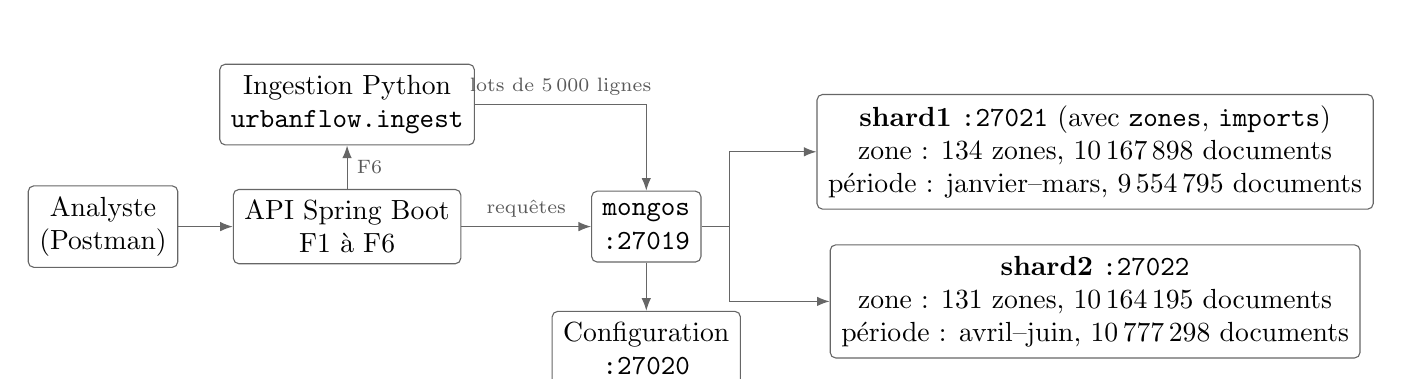
\begin{tikzpicture}[
  every node/.style={align=center},
  box/.style={draw=black!60,rounded corners=2pt,inner sep=4pt,minimum height=9mm},
  link/.style={-{Latex[length=1.6mm]},draw=black!60},
  note/.style={font=\scriptsize,text=black!65}]
\node[box] (client) at (0,0) {Analyste\\(Postman)};
\node[box] (api) at (3.1,0) {API Spring Boot\\F1 à F6};
\node[box] (ingest) at (3.1,1.55) {Ingestion Python\\\code{urbanflow.ingest}};
\node[box] (mongos) at (6.9,0) {\code{mongos}\\\code{:27019}};
\node[box] (config) at (6.9,-1.55) {Configuration\\\code{:27020}};
\node[box,minimum width=6.0cm] (s1) at (12.6,0.95) {\textbf{shard1} \code{:27021} (avec \code{zones}, \code{imports})\\zone : 134 zones, 10\,167\,898 documents\\période : janvier--mars, 9\,554\,795 documents};
\node[box,minimum width=6.0cm] (s2) at (12.6,-0.95) {\textbf{shard2} \code{:27022}\\zone : 131 zones, 10\,164\,195 documents\\période : avril--juin, 10\,777\,298 documents};
\draw[link] (client) -- (api);
\draw[link] (api) -- node[above,note] {requêtes} (mongos);
\draw[link] (api) -- node[right,note] {F6} (ingest);
\draw[link] (ingest.east) -| node[pos=0.25,above,note] {lots de 5\,000 lignes} (mongos.north);
\draw[link] (mongos) -- (config);
\draw[link] (mongos.east) -- ++(0.35,0) |- (s1.west);
\draw[link] (mongos.east) -- ++(0.35,0) |- (s2.west);
\end{tikzpicture}
\caption{Déploiement réparti, avec les documents stockés à six mois. Le déploiement local garde la même API et le même import, avec un seul serveur sur \code{:27018}. Un seul déploiement tourne à la fois, chacun avec ses propres volumes.}\label{fig:architecture}
\end{figure}


\subsection{Ce que fait chaque instance}
\code{explain-requests.py} récupère le pipeline réellement envoyé par l'API et le rejoue
avec \code{explain} sur chaque déploiement \cite{experiences}.

\begin{center}\footnotesize
\begin{tabularx}{\linewidth}{@{}llllX@{}}
\toprule
Requête & Déploiement & Contactés & Documents lus & Sur les shards $\to$ fusion\\
\midrule
Une zone chargée & Local & serveur & 157\,704 & tout sur le serveur\\
(F1, JFK, mars) & Zone & shard2 & 157\,704 & tout sur shard2, sans fusion\\
 & Période & shard1, shard2 & 157\,704 / 0 & \code{$match}, \code{$project} $\to$ \code{$facet}\\
\midrule
Plusieurs zones & Local & serveur & 189\,938 & tout sur le serveur\\
(F2, 5 zones, semestre) & Zone & shard1, shard2 & 88\,485 / 101\,453 & \code{$match}, \code{$project}, \code{$group} $\to$ \code{$group}\\
 & Période & shard1, shard2 & 86\,743 / 103\,195 & idem\\
\midrule
Origine--destination & Local & serveur & 4\,119\,933 & tout sur le serveur\\
(F5, ville, autour & Zone & shard1, shard2 & 2\,062\,737 / 2\,057\,196 & \code{$match}, \code{$project}, \code{$group} $\to$ \code{$group}\\
du 1\textsuperscript{er} avril) & Période & shard1, shard2 & 3\,245\,508 / 874\,425 & idem\\
\bottomrule
\end{tabularx}
\end{center}

Pour F2 et F5, chaque shard regroupe ses documents et n'envoie que des comptes partiels ;
le plan de fusion est \code{$mergeCursors} puis \code{$group}, sur un shard choisi par
MongoDB (\code{anyShard}), et Java combine ensuite les comptes reçus. Sur F2 cinq zones
en placement par zone, les shards émettent 11 Mo par appel et \code{mongos} en rend 4,7 à l'API. \code{$facet}
n'est pas découpé : en placement par période, F1 sur JFK fait sortir 34 Mo par appel de
shard1, contre moins de 0,1 Mo depuis l'unique shard du placement par zone, qui exécute
tout le pipeline sur place.

\subsection{Comparaison automatique}
\code{compare-deployments.py} compare 13 réponses : les huit requêtes de E2 et cinq
requêtes de F1 à F5 qui traversent le 1\textsuperscript{er} avril, plusieurs zones ou les
deux. Les clés JSON sont triées. Les listes gardent l'ordre des services, qui
départagent les ex æquo par identifiants, donc une valeur ou un rang différent fait
échouer le script. Les 13 réponses sont identiques sur les trois déploiements. Une empreinte par fichier (documents, somme des distances, somme des
montants) confirme aussi que les trois bases contiennent les mêmes totaux
\cite{experiences}.

\subsection{Perte d'une instance}
\code{lose-instance.py} arrête un shard, appelle F1 sur la zone 181 à l'arrivée sur le
semestre, dont les trajets sont sur les deux shards, puis F5 sur la ville. Sans shard1 ou
sans shard2, sur les deux placements, l'utilisateur reçoit en 15 à 19 s une erreur 503 :
« MongoDB indisponible ou requête interrompue. Aucun résultat complet ne peut être
fourni. » Le script compare toute réponse 200 à une référence prise sans panne et échoue
si elle diffère.

Shard2 arrêté, une requête limitée à shard1 répond encore 200, à l'identique, parce
qu'elle ne dépend pas de shard2 : zone 1 au départ (placement par zone), zone 181 en
janvier (placement par période). Shard1 arrêté, ces requêtes échouent aussi, parce que
\code{zones} et \code{imports} sont sur ce shard. Après le redémarrage, toutes les
réponses redeviennent identiques à la référence.

Notre déploiement ne récupère donc rien pendant la panne : il n'existe aucune copie, et
les données reviennent seulement avec le shard et son volume. Un système de production
avec des replica sets de plusieurs membres pourrait élire un nouveau primaire et
continuer à répondre ; nous ne l'avons ni déployé ni testé. Nos shards sont aussi deux
conteneurs sur un même PC, dont les pannes ne sont pas indépendantes comme sur des
machines séparées.

\section{Expériences}\label{sec:experiences}
\subsection{Protocole}
Toutes les mesures viennent d'une seule exécution de \code{run-all.py} \texttt{-{}-reset} sur le
code final : 19 étapes réussies en 2 h 01, une seule à la fois et avec un seul
déploiement allumé \cite{experiences}. La machine est un Ryzen 5 7600 (6 cœurs, 12 threads)
avec 32 Go de mémoire et un SSD, sous Windows 11. Docker 28.5.1 sur WSL2 voit 12 CPU et
16,4 Go. Les versions sont MongoDB 8.0.16, Python 3.12.10 et l'API compilée pour Java 21,
exécutée sous Java 24.0.1 avec \code{-Xmx768m}. Le cache WiredTiger est fixé à 1,4 Go en
local et à 0,7 Go par shard, pour garder le même cache total ; les conteneurs n'ont pas d'autre limite. Jenkins tournait
aussi sur le PC, sans que nous mesurions sa consommation. Les temps sont ceux vus par un
client HTTP de l'API. Les paramètres exacts de chaque requête sont dans
\chemin{scripts/common.py} et dans les fichiers de résultats.

\subsection{E1 : volume et chargement}
Les jeux sont cumulés et mesurés en local pendant le chargement. Les « trajets distincts »
sont les lignes du profil activity, donc sans montant négatif ni doublon exact. Chaque
latence est la médiane de cinq appels après un échauffement ; l'écart-type le plus grand
vaut 0,67 s.

\begin{center}\small
\begin{tabular}{lrrr}
\toprule
 & 1 mois & 3 mois & 6 mois\\
\midrule
Lignes sources & 2\,964\,624 & 9\,554\,778 & 20\,332\,093\\
Trajets distincts & 2\,929\,120 & 9\,438\,882 & 20\,074\,661\\
Ingestion cumulée (s) & 90,4 & 302,8 & 652,6\\
Données / index (Mo) & 346,7 / 492,9 & 1\,116,2 / 1\,213,8 & 2\,378,0 / 2\,480,5\\
\midrule
F1 JFK, janvier (s) & 1,588 & 1,629 & 1,572\\
F3 Brooklyn, janvier (s) & 12,819 & 11,376 & 11,203\\
F4 JFK $\to$ Midtown, janvier (s) & 0,050 & 0,045 & 0,043\\
F5 Brooklyn, janvier (s) & 0,253 & 0,258 & 0,266\\
F2 Brooklyn, janvier (s) & 2,010 & 8,269 & 19,487\\
\midrule
F1 zone 181, toute la base (s) & 0,017 & 0,056 & 0,163\\
F2 Brooklyn, toute la base (s) & 2,019 & 10,254 & 25,509\\
\bottomrule
\end{tabular}
\end{center}

Chaque mois s'importe à un rythme de 30\,000 à 33\,000 lignes par seconde. Quand la base
est multipliée par 6,9, les requêtes sur janvier de F1, F3, F4 et F5 ne ralentissent pas.
F2 sur janvier est l'exception, avec un temps multiplié par 9,7. Son filtre combine la date
de départ et un \code{$or} sur les zones de départ et d'arrivée. Or l'index d'arrivée
contient la date d'arrivée : il ne borne pas la date de départ, et nous en déduisons que MongoDB relit les arrivées à Brooklyn de toute la base avant de filtrer ; nous n'avons pas enregistré le plan de cette requête. Nous n'avons pas mesuré d'index
corrigé.

À six mois, l'ingestion dure 652,6 s en local, 646,8 s en zone et 783,2 s en période. Les
données pèsent 2,4 Go partout, mais les index passent de 2,5 Go en local à 4,5 Go en zone
et 5,0 Go en période, pour un total de 4,9, 6,9 et 7,4 Go. Nous n'avons établi la cause ni
de ce surcoût d'index ni du chargement plus lent en période.

\subsection{E2 : local et réparti}\label{sec:e2}
Les données sont celles de six mois. Avant chaque série, les serveurs redémarrent, ce qui
vide le cache de MongoDB mais pas le cache disque de la VM. Chaque requête reçoit un premier
appel, un échauffement, puis cinq appels mesurés avec un seul client.

\begin{center}\footnotesize
\begin{tabular}{@{}l*{3}{r}rrr@{}}
\toprule
 & \multicolumn{3}{c}{Médiane en s (écart-type)} & \multicolumn{3}{c}{Milliers de documents lus par appel}\\
\cmidrule(lr){2-4}\cmidrule(l){5-7}
Requête & Local & Zone & Période & Local & Zone s1/s2 & Période s1/s2\\
\midrule
F1 JFK, départs, mars & 1,584 (0,327) & 1,444 (0,202) & 1,808 (0,355) & 158 & 0 / 158 & 158 / 0\\
F1 zone 181, arrivées, semestre & 1,309 (0,050) & 0,790 (0,028) & 0,843 (0,074) & 50 & 23 / 27 & 24 / 26\\
F2 cinq zones, semestre & 5,396 (0,110) & 3,270 (0,049) & 3,524 (0,226) & 190 & 89 / 101 & 87 / 103\\
F2 Brooklyn, trimestre & 20,976 (0,196) & 13,261 (0,169) & 12,545 (0,132) & 818 & 358 / 460 & 397 / 0\\
F3 Brooklyn, mars & 28,008 (1,006) & 19,231 (0,351) & 35,586 (0,370) & 7\,321 & 3\,664 / 3\,657 & 7\,321 / 0\\
F4 JFK $\to$ Midtown & 0,074 (0,025) & 0,095 (0,015) & 0,098 (0,033) & 4 & 0 / 4 & 4 / 0\\
F5 Brooklyn, mars & 1,930 (0,141) & 1,445 (0,039) & 2,762 (0,046) & 92 & 40 / 52 & 92 / 0\\
F5 ville, autour d'avril & 38,145 (0,854) & 21,877 (1,364) & 59,115 (1,501) & 4\,120 & 2\,063 / 2\,057 & 3\,246 / 874\\
\bottomrule
\end{tabular}
\end{center}

Sur une zone ciblée, les écarts restent petits : pour F1 JFK, ils sont du même ordre que
les écarts-types. Sur les requêtes larges, le temps suit le shard le plus chargé. Pour F5
ville, l'\code{explain} donne 54,7 s à shard1 sur les 59,2 s du placement par période, où ce
shard lit 3\,246 milliers de documents. Le placement par zone coupe la lecture en deux
parts égales et gagne 43\,\% sur le local. Le CPU total des instances pour les cinq appels
vaut 209 s en local, 220 s en zone et 344 s en période.


\begin{itemize}
\item \textbf{Parallélisme.} Sur F2 cinq zones, les deux shards lisent les mêmes documents
que le local à eux deux. Le temps baisse de 39\,\% en zone et le CPU total reste presque
stable (30,2 s puis 31,1 s).
\item \textbf{Cache réduit.} Sur F3 et F5 Brooklyn en période, seul shard1 lit, et il lit
autant que le local, avec 0,7 Go de cache au lieu de 1,4. Les temps augmentent de 27\,\% et
43\,\%, alors que \code{mongos} consomme au plus 0,25 s de CPU. Sur F5 ville, le CPU par
document vaut 10,1 µs en local et 10,6 µs en zone, où le rapport entre documents et cache
est le même, contre 18,9 µs sur shard1 en période, qui lit 1,6 fois plus pour le même cache.
Le cache est la cause probable, mais nous n'avons pas relevé de compteur d'éviction.
\item \textbf{Données réduites.} Sur F2 Brooklyn en période, shard1 lit 397 milliers de
documents contre 818 ailleurs. Comme il ne contient que janvier--mars, l'index d'arrivée
n'y trouve que ces trajets (voir E1). Le gain de 40\,\% vient donc de cette réduction et
pas d'un parallélisme : shard2 ne lit rien.
\end{itemize}
Le premier appel après redémarrage coûte peu : F5 ville prend 38,6 s contre 38,1 s en local,
F1 JFK 2,6 s contre 1,6 s. Ces temps n'ont pas la valeur d'une vraie lecture à froid, puisque
le cache disque de la VM reste plein.

\subsection{E3 : charges contrastées}
La charge A vise quatre zones très actives (F1 au départ et F4 sur une semaine). La charge B
couvre des zones et des périodes variées (F1 à l'arrivée sur le semestre, F2 sur quatre
semaines, F5 avec cinq semaines d'historique, sur Brooklyn et Queens). Chaque mélange compte
60 requêtes envoyées par trois clients, après une passe d'échauffement. La graine est fixe :
un mélange rejoue les mêmes requêtes sur chaque déploiement, mais pas celles d'un autre
mélange. Il n'y a eu qu'un passage par mélange et aucune erreur : la table ne donne donc pas
de variabilité, et nous lisons comme une égalité les écarts de quelques pour cent.

\begin{center}\footnotesize
\begin{tabular}{@{}lrrrrrrrrrrr@{}}
\toprule
 & \multicolumn{3}{c}{Durée totale (s)} & \multicolumn{3}{c}{Médiane A (s)} & \multicolumn{3}{c}{Médiane B (s)} & \multicolumn{2}{c}{CPU s1 / s2 (s)}\\
\cmidrule(lr){2-4}\cmidrule(lr){5-7}\cmidrule(lr){8-10}\cmidrule(l){11-12}
A / B & Local & Zone & Pér. & Local & Zone & Pér. & Local & Zone & Pér. & Zone & Pér.\\
\midrule
60 / 0 & 9,5 & 7,9 & 17,0 & 0,496 & 0,418 & 0,608 & --- & --- & --- & 9 / 12 & 38 / 12\\
42 / 18 & 71,9 & 50,9 & 50,5 & 0,574 & 0,656 & 0,677 & 2,524 & 1,984 & 2,207 & 101 / 130 & 98 / 83\\
18 / 42 & 153,6 & 102,4 & 104,1 & 0,410 & 0,442 & 0,701 & 7,947 & 5,461 & 5,704 & 230 / 276 & 163 / 169\\
0 / 60 & 203,4 & 146,2 & 135,6 & --- & --- & --- & 7,287 & 6,020 & 6,439 & 355 / 425 & 190 / 311\\
\bottomrule
\end{tabular}
\end{center}

\begin{figure}[!htbp]\centering
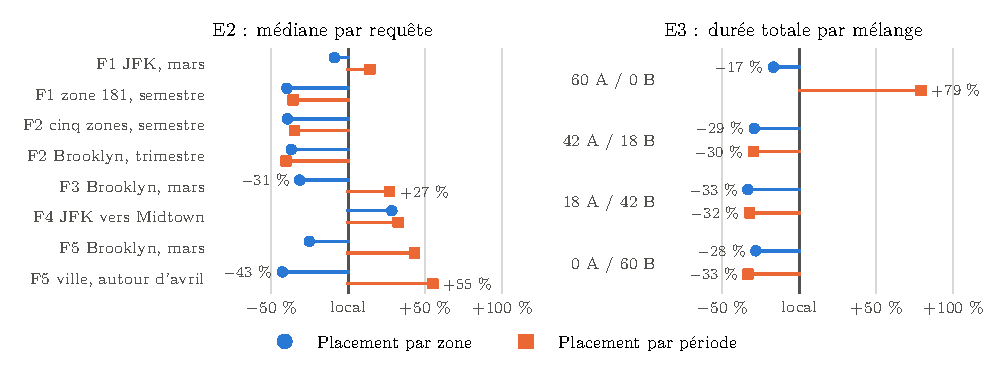
\includegraphics[width=\linewidth]{figures/temps-par-rapport-au-local.pdf}
\caption{Écart de temps de chaque placement par rapport au serveur local : à gauche du trait « local », le placement est plus rapide. Sur F4 et F1 JFK, l'écart reste petit en valeur absolue ou proche de la variabilité.}\label{fig:temps}
\end{figure}

Nous avons écrit la prédiction avant les mesures \cite{prediction}.
\begin{itemize}
\item \textbf{Faux : le local est le plus rapide sur A.} Le placement par zone termine en
7,9 s contre 9,5 s. Nous attendions un surcoût de \code{mongos} et du cache coupé en deux.
Or \code{mongos} consomme 0,3 s de CPU, et les zones chaudes sont séparées (568 et 797
milliers de documents) : la charge ne se concentre pas sur un shard. Le local garde une
médiane A un peu plus basse dans les deux mélanges intermédiaires.
\item \textbf{Juste, avec une erreur d'ampleur : la zone est le meilleur placement réparti
sur A.} Nous attendions un écart faible, et il va du simple au double (7,9 s contre 17,0 s).
Les 12 appels F4 dont toute la fenêtre tombe sur shard1 prennent 1,3 à 3,0 s en période, contre
au plus 0,65 s pour les 17 autres et jamais plus de 0,58 s en zone. Sur tout le mélange, shard1 lit 6,8 millions
de clés pour 1,1 million de documents. Le même F4 n'était pas lent dans E2 (0,098 s). Nous n'avons pas enregistré les plans pendant E3 : un mauvais choix d'index sur shard1 reste une hypothèse.
\item \textbf{Juste : le réparti gagne 20 à 40\,\% sur B.} La durée baisse de 28\,\% en zone et
33\,\% en période.
\item \textbf{Faux : F1 reste plus lent en réparti à cause de \code{$facet}.} Dans E2, F1 sur la
zone 181 descend de 1,309 s à 0,790 et 0,843 s. La lecture, faite en parallèle avant la fusion,
semble peser plus que \code{$facet}.
\item \textbf{À moitié juste : la période bat la zone sur B.} Elle gagne en durée totale (135,6 s
contre 146,2 s), mais pas en médiane (6,439 s contre 6,020 s). Sa durée profite des F2 longs,
médiane 12,8 s contre 15,2 s. Elle lit aussi moins de documents, 19,3 millions contre 25,4.
\item \textbf{Faux : le meilleur choix bascule du local au réparti au milieu du mélange.} Le
local ne gagne aucun mélange en durée totale (figure~\ref{fig:temps}) : la zone est devant dès 60 / 0, et zone et période
sont à égalité dans les deux mélanges intermédiaires.
\item \textbf{Juste : la charge est déséquilibrée en période quand les requêtes visent un
trimestre.} Sur A, shard1 consomme 38 s de CPU et shard2 12 s, contre 9 et 12 s en zone.
\end{itemize}

En zone, le temps gagné se paie en ressources. Sur 0 / 60, le CPU total passe de 628 s en local à
787 s, \code{mongos} compris ; il descend à 508 s en période, qui lit moins. Le serveur local
émet 168 Mo ; les shards en émettent 1\,231 en zone et 1\,094 en période, à cause des
résultats partiels et de la fusion. La mémoire relevée à la fin passe de 2,2 Go à 2,7 Go.

Pour des requêtes ciblées fréquentes et des analyses de la ville occasionnelles, nous
retiendrions le placement par zone : il arrive premier ou à égalité sur trois mélanges sur quatre,
il répartit le travail de façon régulière et il évite les 59 s de F5 ville. Il perd 7\,\% face
à la période sur 0 / 60 et coûte 42\,\% de stockage de plus que le local. Nous n'avons pas réalisé l'expérience bonus E4.

\section{Vérifications et limites}\label{sec:verifications}
\subsection{Vérifications indépendantes}
Les scripts relisent les Parquet avec Pandas sans utiliser les comptes de MongoDB, puis comparent
leur calcul à la réponse de l'API. Les fichiers sont dans \chemin{results/verification/}.
\begin{itemize}
\item \textbf{Janvier, base temporaire.} \code{verify-f2} à \code{verify-f5-parquet.py} réussissent
sur F2 (zone 181, Brooklyn avec 25\,258 candidats et 24\,860 retenus), F3 (zone 132, Brooklyn avec
3 cellules inhabituelles sur 610), F4 (132 $\to$ 161, 161 $\to$ 236, échantillon insuffisant pour
181 $\to$ 89) et F5 (zone 132, Brooklyn, ville avec 19\,368 paires). Nous avons lancé ce contrôle le 7 novembre, lors de l'essai complet sur janvier et avril. Le code de l'API et de l'ingestion est
le même que dans la version finale, seuls des scripts ayant changé entre les deux.
\item \textbf{Six mois, base complète.} \code{verify-registered-period.py} retrouve F1 sur la zone
181 à l'arrivée (50\,064 candidats, 49\,616 retenus), F2 sur Brooklyn de janvier à mars (97\,219 et
95\,809), F4 de JFK à Midtown autour du 10 mars (1\,792 et 2\,220 trajets, médianes 2\,963,5 et
3\,086,5 s) et les trajets d'avril vus par F6.
\item \textbf{Traçabilité.} \code{verify-trips.py} vérifie que \code{/api/trips} renvoie pour la zone
181 les mêmes comptes que F1 (983 candidats, 977 retenus) avec le bon fichier source.
\item \textbf{Changement d'heure.} \code{verify-f4-dst.py} retrouve les 10\,891 s de la ligne
942\,762 de mars et la durée absente de la ligne 841\,170. Il porte sur ces deux lignes réelles
dans une base temporaire et ne valide pas le mois entier.
\end{itemize}
Les archives de chaque benchmark de la section~\ref{sec:mesures} enregistrent aussi des réponses
JSON identiques avant et après index.

\subsection{Limites}
\begin{itemize}
\item Tous les processus partagent le CPU, la mémoire et le disque d'un même PC. Les gains de E2 et
E3 ne se transposent pas à des machines indépendantes, où le réseau compterait et où les disques ne
seraient plus partagés.
\item Les mesures de E1 et E2 reposent sur cinq appels et celles de E3 sur un seul passage. Jenkins
tournait pendant les mesures.
\item Les mesures de la section~\ref{sec:mesures} viennent d'un serveur Linux à deux CPU, sur janvier
et avant les optimisations de F3 et F5. Elles justifient les index, mais ne se comparent pas à E1--E3.
L'index \code{pickup_datetime_zone} n'a pas de mesure séparée.
\item Trois causes restent à établir : le surcoût d'index en réparti, le chargement plus lent en
période et les F4 lents sur shard1 dans E3.
\item Les seuils statistiques restent descriptifs, les calendriers sont incomplets pour les événements
locaux et les flags ne détectent pas toute anomalie. 
\end{itemize}

\begin{thebibliography}{9}\small
\bibitem{sujet} H. Akid, \emph{Project 3 --- UrbanFlow, An Urban Mobility Analytics Platform}, Big Data and NoSQL, M2 SLCD, Université Côte d'Azur, 2026--2027.
\bibitem{tlc} NYC TLC, \emph{Trip Record Data} et référentiel officiel. URLs et dates de récupération consignées dans \chemin{data/manifest.json}. \url{https://www.nyc.gov/site/tlc/about/tlc-trip-record-data.page}.
\bibitem{code} UrbanFlow, version finale du code, 7 novembre 2026 : \chemin{urbanflow/ingest.py}, \chemin{urbanflow/deploy.py}, \chemin{backend/src/main/java/fr/urbanflow/}. \url{https://github.com/deliasTheo/UrbanFlow-noSQL}.
\bibitem{preuves} UrbanFlow, manifeste, rapport qualité et bilans d'import : \chemin{data/manifest.json}, \chemin{results/quality/quality_report.json}, \chemin{results/ingestion/2024-01.json} à \chemin{2024-06.json}.
\bibitem{experiences} UrbanFlow, exécution finale du 7 novembre 2026 : \chemin{results/experiments/} (E1--E3, environnement, journal \chemin{run-all.json}), \chemin{results/distributed/} (comparaison, plans, pannes, placement), \chemin{results/verification/}.
\bibitem{prediction} UrbanFlow, prédiction de E3 écrite avant les mesures : \chemin{docs/prediction-e3.md}.
\bibitem{mesures} UrbanFlow, mesures initiales du 5 novembre 2026 : \chemin{results/performance/f1-indexes.md} et répertoires \chemin{results/performance/f2/} à \chemin{f5/}, notamment \code{measurements.json}, réponses, plans et vérifications.
\bibitem{calendrier} U.S. Office of Personnel Management, \emph{2024 Federal Holidays}. Calendrier repris dans \chemin{backend/src/main/java/fr/urbanflow/unusual/Calendar2024.java}. \url{https://www.opm.gov/policy-data-oversight/pay-leave/federal-holidays/}.
\end{thebibliography}

\label{fin-corps}
\clearpage\appendix
\section{Anomalies présentes et lignes justificatives}\label{ann:qualite}
Fréquences issues de \chemin{results/quality/quality_report.json}, calculées
\emph{par fichier entier}, indépendamment des profils. Elles peuvent se recouper.
Nous avons comparé les huit exemples aux colonnes originales des Parquet et recalculé leurs durées avec New York puis UTC. Le relevé de cette vérification est
\chemin{report/evidence-verification.json}. Une transition DST est une particularité
à traiter, pas nécessairement une erreur de données. Les numéros de ligne sont en base zéro.

\begin{center}\small
\begin{tabular}{llrr}
\toprule
Mois & Indicateur & Fréquence & Part du fichier (\%)\\
\midrule
2024-01 & \code{PICKUP_OUTSIDE_FILE_MONTH} & 18 & 0,000607\\
2024-01 & \code{NON_POSITIVE_DURATION} & 870 & 0,029346\\
2024-01 & \code{ZERO_DISTANCE} & 60\,371 & 2,036380\\
2024-01 & \code{NEGATIVE_AMOUNT} & 35\,504 & 1,197589\\
2024-01 & \code{UNKNOWN_ZONE} & 31\,527 & 1,063440\\
2024-02 & \code{EXACT_DUPLICATE} & 1 & 0,000033\\
2024-03 & \code{DST_SPANNING} & 1\,153 & 0,032183\\
2024-03 & \code{DST_UNRESOLVED} & 3 & 0,000084\\
\bottomrule
\end{tabular}\end{center}

\paragraph{2024-01, ligne 256 --- \code{PICKUP_OUTSIDE_FILE_MONTH}}
Départ : 2023-12-31 23:56:46 ; arrivée : 2024-01-01 00:12:06. Zones 236 $\to$ 142, fournisseur 2, distance 2.38 miles, total 21.6.
Le départ est en décembre alors que la ligne est publiée en janvier ; la requête doit utiliser la date réelle.

\paragraph{2024-01, ligne 87\,994 --- \code{NON_POSITIVE_DURATION}}
Départ : 2024-01-02 10:00:00 ; arrivée : 2024-01-02 09:53:56. Zones 75 $\to$ 95, fournisseur 1, distance 7.2 miles, total 46.94.
L'arrivée précède le départ : durée réelle $-364$ s, exclue du profil journey.

\paragraph{2024-01, ligne 17 --- \code{ZERO_DISTANCE}}
Départ : 2024-01-01 00:52:09 ; arrivée : 2024-01-01 00:52:28. Zones 237 $\to$ 237, fournisseur 2, distance 0.0 miles, total 8.0.
Distance nulle malgré 19 s entre les deux heures : la ligne reste stockée mais n'alimente pas journey.

\paragraph{2024-01, ligne 99 --- \code{NEGATIVE_AMOUNT}}
Départ : 2024-01-01 00:18:24 ; arrivée : 2024-01-01 00:30:39. Zones 249 $\to$ 232, fournisseur 2, distance 2.16 miles, total -18.5.
Le montant total négatif est exclu des profils analytiques. Le rapport qualité repère aussi cette ligne comme écriture d'annulation.

\paragraph{2024-01, ligne 24 --- \code{UNKNOWN_ZONE}}
Départ : 2024-01-01 00:42:05 ; arrivée : 2024-01-01 01:16:49. Zones 263 $\to$ 265, fournisseur 1, distance 23.9 miles, total 127.94.
L'arrivée 265 ne désigne pas une zone précise de New York : exclusion du profil flows et donc journey.

\paragraph{2024-02, ligne 754\,252 --- \code{EXACT_DUPLICATE}}
Départ : 2024-02-08 18:23:50 ; arrivée : 2024-02-08 18:38:14. Zones 162 $\to$ 230, fournisseur 2, distance 0.81 miles, total 23.16.
Le rapport qualité signale cette ligne comme copie d'une ligne précédente du même fichier ; seule la copie est exclue. Les champs cités identifient l'exemple, le rapport JSON conserve toutes les colonnes.
La ligne identique antérieure se trouve à la position 754\,248.

\paragraph{2024-03, ligne 942\,762 --- \code{DST_SPANNING}}
Départ : 2024-03-09 23:38:43 ; arrivée : 2024-03-10 03:40:14. Zones 249 $\to$ 203, fournisseur 2, distance 31.35 miles, total 131.14.
Durée UTC de 10\,891 s contre 14\,491 s locales : une heure est retranchée. Le flag n'exclut pas automatiquement le trajet de journey.

\paragraph{2024-03, ligne 841\,170 --- \code{DST_UNRESOLVED}}
Départ : 2024-03-09 02:31:02 ; arrivée : 2024-03-10 02:09:54. Zones 114 $\to$ 48, fournisseur 2, distance 3.36 miles, total 27.72.
L'arrivée est à une heure inexistante le 10 mars. La durée exploitable est null et non les 85\,132 s de différence locale.

\end{document}
